\documentclass[10pt]{article}
\usepackage{tikz}
\usetikzlibrary{shapes.misc}
\usepackage[margin=0cm]{geometry}
\pagestyle{empty}
\tikzstyle{every node}=[cross out, draw, red]

\begin{document}

\vspace*{\fill}
\begin{center}
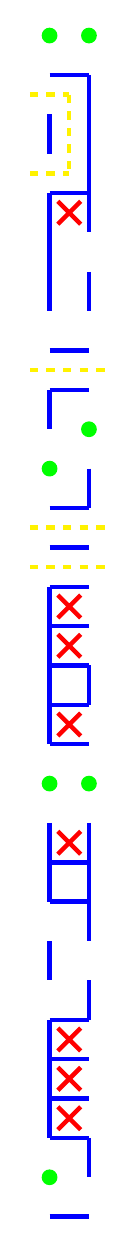
\begin{tikzpicture}[x=0.5cm, y=-0.5cm, ultra thick, blue]
% Walls
    \draw (0,1) -- (1,1);
    \draw (0,4) -- (1,4);
    \draw (0,8) -- (1,8);
    \draw (0,9) -- (1,9);
    \draw (0,12) -- (1,12);
    \draw (0,13) -- (1,13);
    \draw (0,14) -- (1,14);
    \draw (0,15) -- (1,15);
    \draw (0,16) -- (1,16);
    \draw (0,17) -- (1,17);
    \draw (0,18) -- (1,18);
    \draw (0,21) -- (1,21);
    \draw (0,22) -- (1,22);
    \draw (0,25) -- (1,25);
    \draw (0,26) -- (1,26);
    \draw (0,27) -- (1,27);
    \draw (0,28) -- (1,28);
    \draw (0,30) -- (1,30);
    \draw (0,2) -- (0,3);
    \draw (0,4) -- (0,7);
    \draw (0,9) -- (0,10);
    \draw (0,14) -- (0,18);
    \draw (0,20) -- (0,22);
    \draw (0,23) -- (0,24);
    \draw (0,25) -- (0,28);
    \draw (1,1) -- (1,5);
    \draw (1,6) -- (1,7);
    \draw (1,11) -- (1,12);
    \draw (1,16) -- (1,17);
    \draw (1,20) -- (1,23);
    \draw (1,24) -- (1,25);
    \draw (1,28) -- (1,29);
% Pillars
    \fill[green] (0,0) circle(0.2);
    \fill[green] (1,0) circle(0.2);
    \fill[green] (1,10) circle(0.2);
    \fill[green] (0,11) circle(0.2);
    \fill[green] (0,19) circle(0.2);
    \fill[green] (1,19) circle(0.2);
    \fill[green] (0,29) circle(0.2);
% Inner points in accessible cul-de-sacs
    \node at (0.5,4.5) {};
    \node at (0.5,14.5) {};
    \node at (0.5,15.5) {};
    \node at (0.5,17.5) {};
    \node at (0.5,20.5) {};
    \node at (0.5,25.5) {};
    \node at (0.5,26.5) {};
    \node at (0.5,27.5) {};
% Entry-exit paths without intersections
    \draw[dashed, yellow] (-0.5,1.5) -- (0.5,1.5);
    \draw[dashed, yellow] (-0.5,3.5) -- (0.5,3.5);
    \draw[dashed, yellow] (-0.5,8.5) -- (1.5,8.5);
    \draw[dashed, yellow] (-0.5,12.5) -- (1.5,12.5);
    \draw[dashed, yellow] (-0.5,13.5) -- (1.5,13.5);
    \draw[dashed, yellow] (0.5,1.5) -- (0.5,3.5);
\end{tikzpicture}
\end{center}
\vspace*{\fill}

\end{document}
